\chapter{Конструкторская часть}

% В данном разделе представлены этапы проектирования выделенных в предыдущем разделе баз данных, нужных для решения задачи.
\section{Функциональная модель}

На рисунке \ref{img:func_model} изображена функциональная модель, отображающая структуру и функции системы.

\begin{figure}[h!]
	\begin{center}
		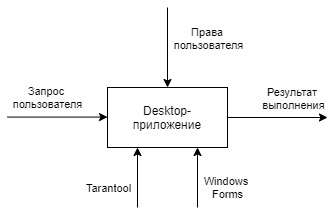
\includegraphics[scale=0.7]{../imgs/func_model.jpg}
	\end{center}
	\captionsetup{justification=centering}
	\caption{Функциональная модель приложения}
	\label{img:func_model}
\end{figure}






\section{Сценарии использования}

Сценарии использования описываются с помощью Use Case Diagram (диаграммы прецедентов). Она состоит из графической диаграммы, описывающей действующие лица и прецеденты – конкретные действия, которые выполняет пользователь при работе с системой.

\clearpage
На рисунке \ref{img:use_case1} представлена Use Case Diagram для действий неавторизованного пользователя.


\begin{figure}[h!]
	\begin{center}
		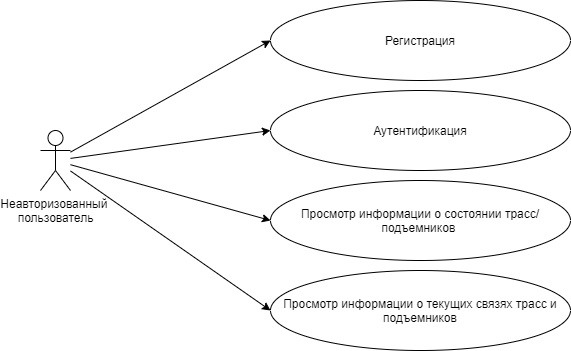
\includegraphics[scale=0.7]{../imgs/use_case/use-case1.png}
	\end{center}
	\captionsetup{justification=centering}
	\caption{Use Case Diagram действий неавторизованного пользователя}
	\label{img:use_case1}
\end{figure}


На рисунке \ref{img:use_case2} представлена Use Case Diagram для действий авторизованного пользователя.

\begin{figure}[h!]
	\begin{center}
		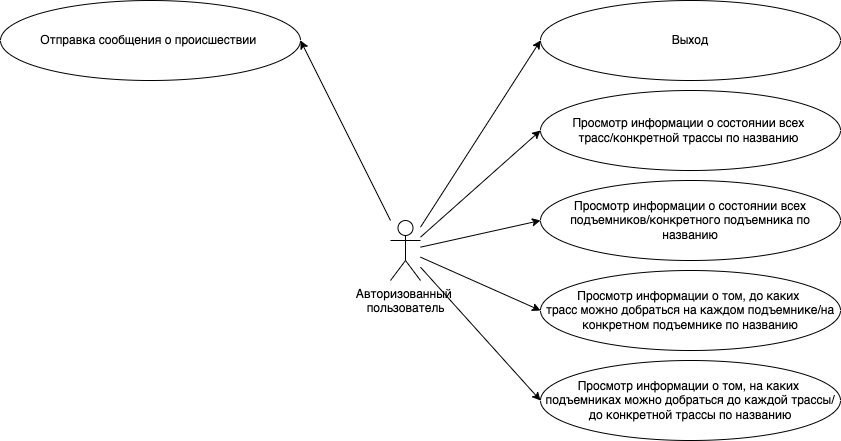
\includegraphics[scale=0.6]{../imgs/use_case/use-case2.png}
	\end{center}
	\captionsetup{justification=centering}
	\caption{Use Case Diagram действий авторизованного пользователя}
	\label{img:use_case2}
\end{figure}


\clearpage
На рисунке \ref{img:use_case3} представлена Use Case Diagram для действий сотрудника лыжного патруля.

\begin{figure}[h!]
	\begin{center}
		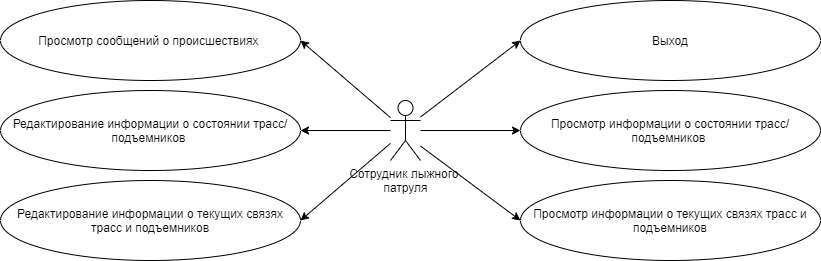
\includegraphics[scale=0.6]{../imgs/use_case/use-case3.png}
	\end{center}
	\captionsetup{justification=centering}
	\caption{Use Case Diagram действий сотрудника лыжного патруля}
	\label{img:use_case3}
\end{figure}


На рисунке \ref{img:use_case4} представлена Use Case Diagram для действий администратора.

\begin{figure}[h!]
	\begin{center}
		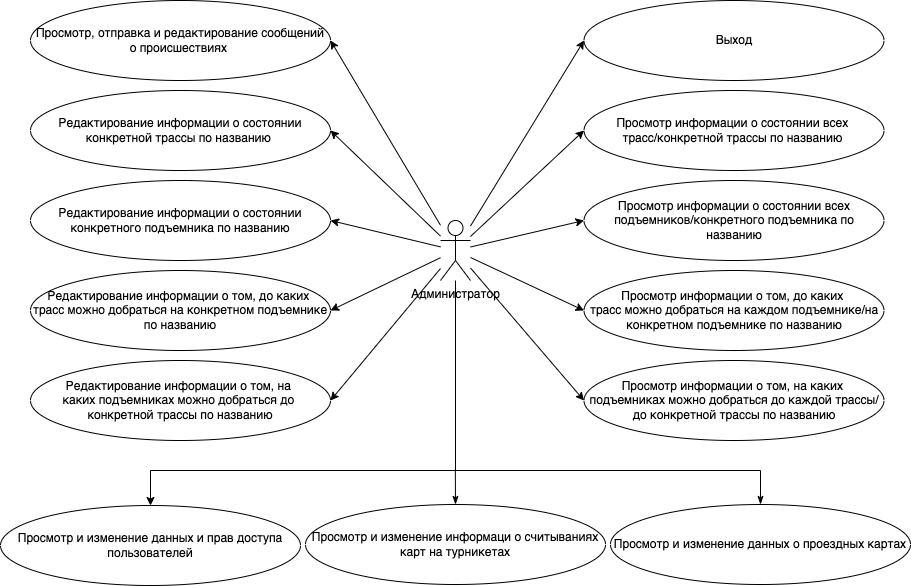
\includegraphics[scale=0.5]{../imgs/use_case/use-case4.png}
	\end{center}
	\captionsetup{justification=centering}
	\caption{Use Case Diagram действий администратора}
	\label{img:use_case4}
\end{figure}



\section{Проектирование базы данных}


На рисунке \ref{img:er} отображена диаграмма сущностей системы. Данная схема построена на основе категорий и сведений о данных, отображенных в таблице \ref{tbl:1}.

\clearpage
\begin{figure}[h!]
	\begin{center}
		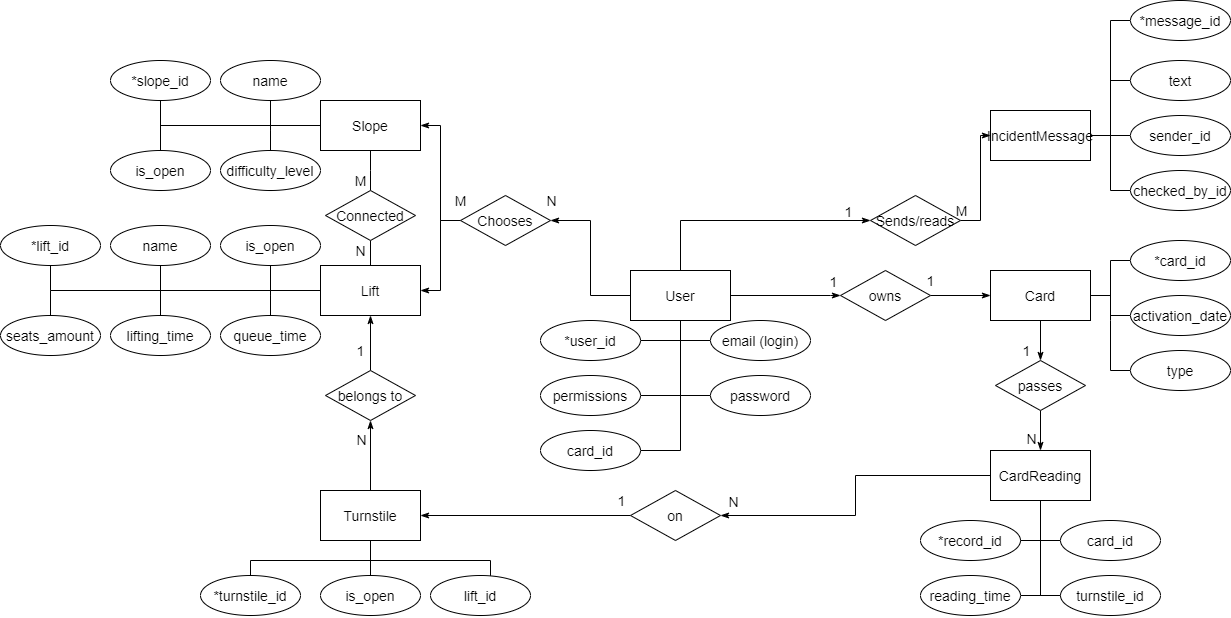
\includegraphics[scale=0.4]{../imgs/er/er.png}
	\end{center}
	\captionsetup{justification=centering}
	\caption{Диаграмма сущностей системы}
	\label{img:er}
\end{figure}

В соответствии с этой диаграммой база данных должна хранить следующие таблицы:  


\begin{itemize}
	\item таблица трасс slopes;
	\item таблица подъемников lifts;
	\item таблица связей трасс и подъемников lifts\_slopes;
	\item таблица турникетов turnstiles;
	\item таблица проездных карт cards;
	\item таблица считываний карт на турникетах подъемников card\_readings;
	\item таблица сообщений о происшествиях messages;
	\item таблица пользователей users.
	%\item таблица групп пользователей.
\end{itemize}


Таблица slopes хранит информацию о трассах и содержит следующие поля:
\begin{itemize}
	\item slope\_id -- уникальный идентификатор трассы, PK;
	\item slope\_name -- уникальное название;
	\item difficulty\_level -- уровень сложности;
	\item is\_open -- открыта или закрыта.
\end{itemize}


Таблица lifts хранит информацию о подъемниках и содержит следующие поля:
\begin{itemize}
	\item lift\_id -- уникальный идентификатор подъемника, PK;
	\item lift\_name -- уникальное название;
	\item is\_open -- открыт или закрыт;
	\item seats\_amount -- количество мест;
	\item lifting\_time -- время подъема;
	\item queue\_time -- время в очереди;
\end{itemize}


Эти две таблицы связаны отношением многие-ко-многим. Таблица lifts\_slopes хранит информацию об этих отношениях (связях трасс и подъемников) и содержит следующие поля:
\begin{itemize}
	\item record\_id -- уникальный идентификатор записи, PK;
	\item lift\_id -- идентификатор подъемника, FK на поле lift\_id таблицы lifts;
	\item slope\_id -- идентификатор трассы, FK на поле slope\_id таблицы slopes.
\end{itemize}


Таблица turnstiles хранит информацию о турникетах и содержит следующие поля:
\begin{itemize}
	\item turnstile\_id -- уникальный идентификатор турникета, PK;
	\item lift\_id -- идентификатор подъемника, FK на поле lift\_id таблицы lifts;
	\item is\_open -- открыт или закрыт.
\end{itemize}


Таблица cards хранит информацию о проездных картах и содержит следующие поля:
\begin{itemize}
	\item card\_id -- уникальный идентификатор карты, PK;
	\item activation\_time -- дата и время активации;
	\item type -- тип карты (детская, взрослая, временная, ...).
\end{itemize}


Таблица card\_readings хранит информацию о считываниях карт на турникетах подъемников и содержит следующие поля:
\begin{itemize}
	\item record\_id -- уникальный идентификатор считывания, PK;
	\item turnstile\_id -- идентификатор турникета, FK на поле turnstile\_id таблицы turnstiles;
	\item card\_id -- идентификатор проездной карты, FK на поле card\_id таблицы cards;
	\item reading\_time -- дата и время считывания.
\end{itemize}


Таблица users хранит информацию о пользователях и содержит следующие поля:
\begin{itemize}
	\item user\_id -- уникальный идентификатор пользователя, PK;
	\item card\_id -- идентификатор проездной карты (может отсутсвовать), FK на поле card\_id таблицы cards;
	\item user\_email -- адрес электронной почты (он же будет использоавться как логин);
	\item password -- пароль;
	\item permissions -- права доступа (роль).
\end{itemize}


Таблица messages хранит информацию о сообщениях пользователей о происшествиях и содержит следующие поля:
\begin{itemize}
	\item message\_id -- уникальный идентификатор сообщения, PK;
	\item sender\_id -- идентификатор отправителя, FK на поле user\_id таблицы usres;
	\item checked\_by\_id -- идентификатор прочитавшего, FK на поле user\_id таблицы usres;
	\item text -- текст сообщения.	
\end{itemize}



На рисунке \ref{img:db} предоставлена диаграмма реализованной базы данных.



\begin{figure}[h!]
	\begin{center}
		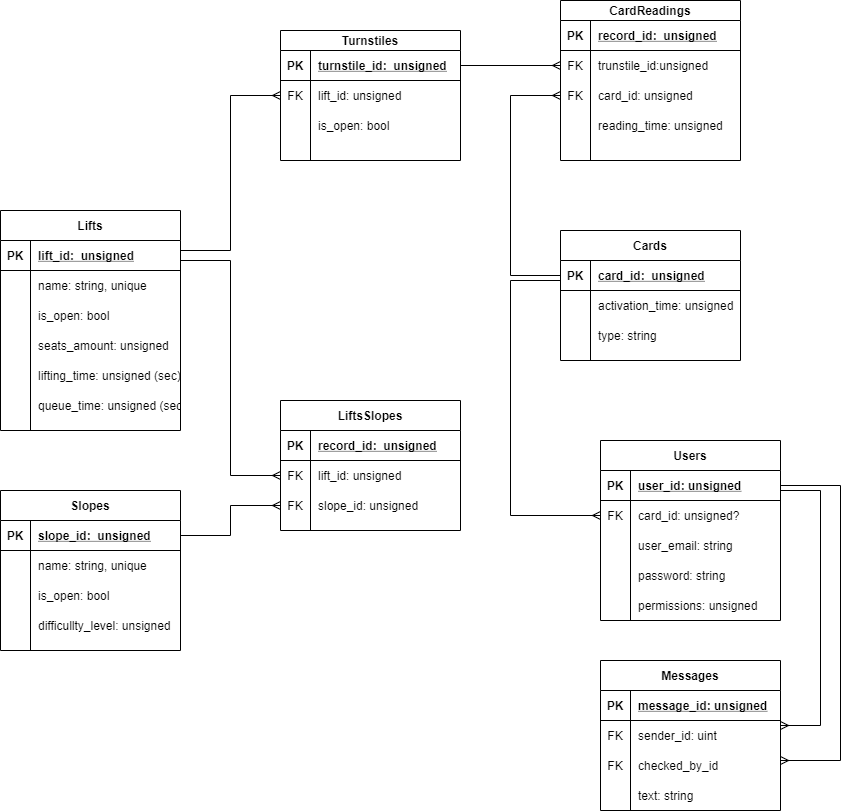
\includegraphics[scale=0.4]{../imgs/db/db.png}
	\end{center}
	\captionsetup{justification=centering}
	\caption{Диаграмма базы данных}
	\label{img:db}
\end{figure}






























!!!!Кроме того, для каждой таблицы будет реализован триггер, срабатывающий после обновления или удаления данных из таблиц. Этот триггер будет посылать сигнал базе данных кэширования, с помощью языка plpython3u, о необходимости обновить или удалить информацию из кэша. С помощью таких триггеров можно решить проблему синхронизации данных в хранилище и кэше.

\section{Проектирование базы данных кэширования}

База данных кэширования будет реализована с помощью использования СУБД Tarantool. В базе данных будут полностью продублированны таблицы (в виде спейсов) из хранилища рабочих программ дисциплин. Первичным ключом будет являться поле с уникальным идентификатором этих таблиц (\texttt{id}). Кроме того, для спейсов хранящих поле \texttt{discipline\_id} будет добавлен вторичный ключ по этому полю, для удобного и быстрого сбора нужных данных по заданной дисциплине.

При запросе данных у приложения, будет проводиться проверка, присутствует ли запись в кэше. Если запись присутствует, запрос к базе данных рабочих программ дисциплин производиться не будет и будут возвращены данные из кэша. В противном случае, будет произведен запрос к базе данных хранящую информацию о дисциплинах.

Все спейсы будут созданы на основе движка \texttt{memtx}, хранящего все данные в оперативной памяти. Персистентность данных будет обеспечивается при помощи ведения журнала транзакция и системы <<снимков>> текущего состояния кэша. Эти технологии помогут решить проблему <<холодного>> старта базы данных кэширования.

\section*{Вывод}

В данном разделе были представлены этапы проектирования баз данных и рассмотрены особенности используемых СУБД на архитектурном уровне.
